\newpage

\section{Abbildungsverzeichnis}
%urls with "%" in the url fail the build
%escape the symbols with "\" ("\%") or try shorter urls
%for example:
%https://www.ac-illust.com/main/detail.php?id=971750&word=%E3%81%8B%E3%82%8F%E3%81%84%E3%81%84%E3%82%BF%E3%82%B3%E3%81%95%E3%82%93%E3%82%A6%E3%82%A4%E3%83%B3%E3%83%8A%E3%83%BC
%can be shortend to https://www.ac-illust.com/main/detail.php?id=971750 and still works

\begin{figure}[ht]
	\centering
	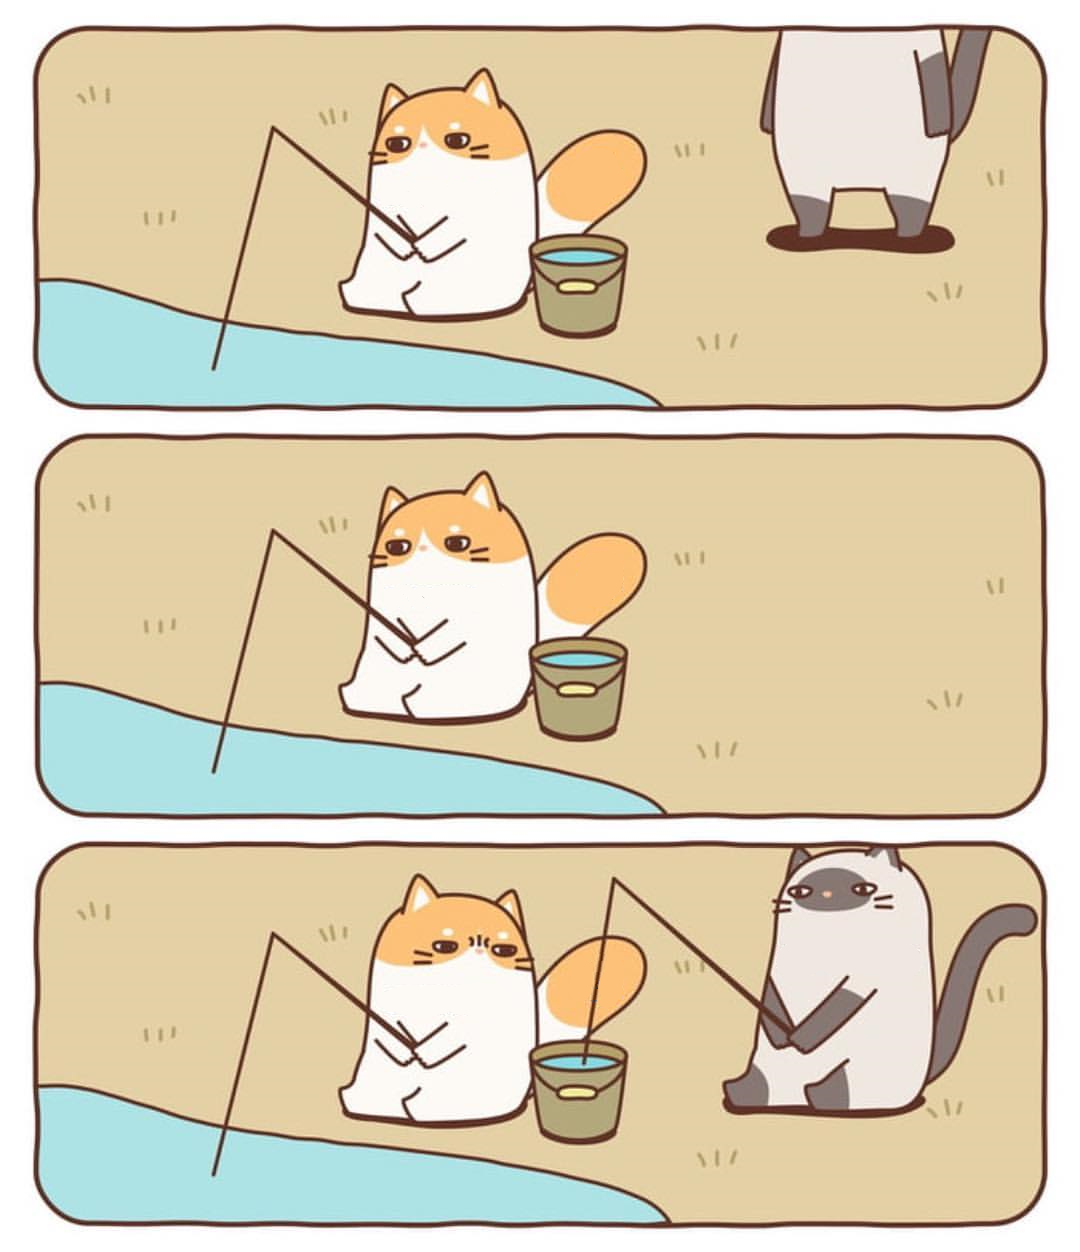
\includegraphics[width=.9\linewidth]{pictures/cat.png}
	\caption{\textsl{Diebstahl in der Fischerei}.
    Unbekannt \textsc{Unbekannt}. 2019. imgflip.  \url{https://imgflip.com/memetemplate/190870186/Catfishing} (Letzter Abruf: 11.11.2023). S. 1. Die Breite der Bilder (und damit die Größe) kann man bei width ändern}
	\label{fig:Diebstahl in der Fischerei}
\end{figure}

\begin{figure}[ht]
	\centering
	
\includegraphics[width=\linewidth]{pictures/tako.png}
	\caption{\textsl{Kawaii tako}.
    Nogie \textsc{Tako-san}. 2019. imgflip. 
    \url{https://www.ac-illust.com/main/detail.php?id=971750} (Letzter Abruf: 11.11.2023). S. 1}
	\label{fig:Kawaii Tako}
\end{figure}
